\chapter{Représentation des cartes de Kohonen}
\graphicspath{{03-Representation/}}

\minitoc
\section{Problématique}

Les cartes de Kohonen sont généralement associées à une facilité de représentation et de visualisation. En effet, leur nombre réduit de prototypes et leur aspect topologique permet d'en tracer une représentation visuselle facilement interprétable. Cette facilité d'interprétation, cependant, est limitée à un domaine d'utilisation : celui dans lequel les éléments qui nous intéressent sont les distances euclidiennes entre les données, ou plus généralement dans lequel la distance considérée pour la mise a jour des cartes possède un pendant graphique directement interprétable à l'oeil humain. Dans un cas plus général de cartes auto-organisatrices, telles que celles agissant dans CxSOM, l'apprentissage repose sur des calculs d'activités et un processus de relaxation. Ces activités n'ont pas forcément un pendant graphique. De ce fait, leur représentation graphique mérite une analyse plus approfondie que dans le cas de cartes classiques. 

\subsection{Représentation classique des cartes de Kohonen}

La manière la plus répandue de représenter une carte de Kohonen est de tracer les poids de ses prototypes, disposés dans le graphe qu'est la carte. En fonction des dimensions des entrées, cette représentation prennent plusieurs formes. Deux exemples courants de représentation sont les suivants: 
\begin{itemize}
\item Le graphe qu'est la carte de Kohonen est représenté dans l'espace de ses positions (la grille d'indices $(i,j)$, ou une ligne indexée par $i$. Sur chaque noeud est tracé le poids correspondant. C'est le cas par exemple en figure~\ref{fig:digits} dans lequel les poids des prototypes, qui sont des imagettes, sont affichés en chaque point de la grille. Si la dimension d'un poids est trop grande pour être représentée graphiquement, il est également courant de labeliser chaque prototype et d'afficher ces labels sur les noeuds de la carte, en tant que représentation.
\item Lorsque les données traitées sont des points deux ou trois dimensions, les poids des prototypes peuvent être directement tracés dans l'espace $R^2$ ou $R^3$. Ces poids sont alors reliés en fonction des positions des noeuds dans la carte, montrant ainsi la déformation de la carte dans l'espace d'entrée, c'est le cas en figure~\ref{fig:points2D}.
\end{itemize}

\begin{figure}
\begin{minipage}{0.5\textwidth}
\centering
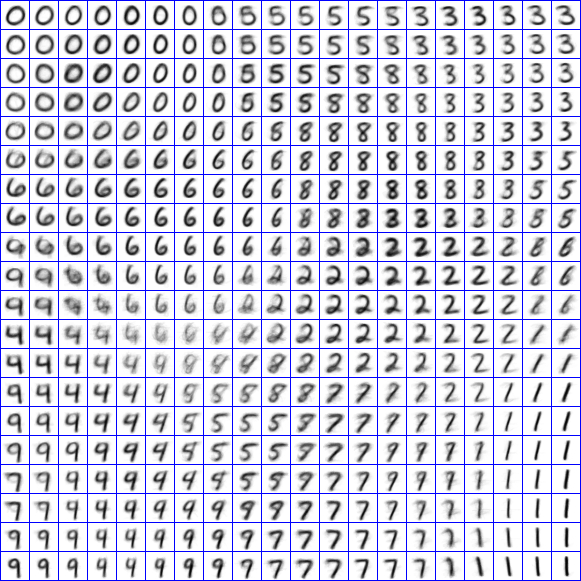
\includegraphics[width=0.5\textwidth]{digits.jpg}
\label{fig:digits}
\end{minipage}
\begin{minipage}{0.5\textwidth}
\centering
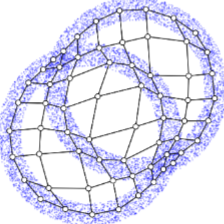
\includegraphics[width=0.5\textwidth]{points.png}
\label{fig:points2D}
\end{minipage}
\caption{Représentations possible des poids d'une carte de Kohonen classiques, dans le cas d'entrées sous forme d'imagettes ou de points en deux dimensions.}
\end{figure}

Ces représentations sont particulièrement adaptées à un observateur humain. Il est ainsi alors facile de labeliser les prototypes, de visualiser les clusters ... Ceci étant conditionné à ce que les cartes se soient organisées en suivant une distance. Lorsqu'il regarde la carte, l'oeil humain se demande : "est-ce que la carte est bien dépliée sur toutes les données ? Est-ce qu'un prototype représente correctement une donnée ?" Intellectuellement, il imagine en fait une donnée, par exemple une imagette d'un chiffre à main levée, et reproduit le processus de sélection du BMU qui a eu lieu lors de l'apprentissage de la carte pour trouver le poids qui lui correspond le mieux. 

\subsection{Limites de cette représentation dans CxSOM}

Dans CxSOM, le choix du BMU se fait suivant plusieurs activités, et plus encore, suivant un processus de relaxation. Il est bien entendu possible de tracer les poids d'une carte après apprentissage, comme représenté en figure~\ref{fig:weights}. Cependant, le processus intellectuel menant à la représentation mentale d'une carte, en regardant les poids, n'est plus possible. En imaginant une donnée, on ne pourra pas trouver le BMU selectionné. La simulation du processus d'activité et relaxation est nécessaire pour la représentation compréhensible par l'humain d'une carte au sein de CxSOM. Par ailleurs, chaque unité d'une carte a plusieurs poids. Il est donc compliqué de comprendre directement le rôle de ces poids en regardant leur valeur.
\begin{figure}
\centering
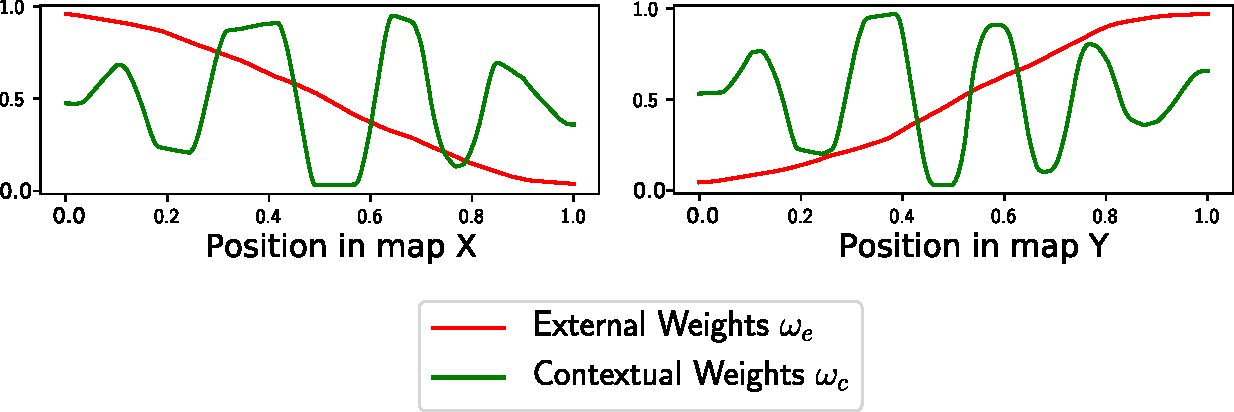
\includegraphics[width=0.7\textwidth]{weights_2.pdf}
\label{fig:weights}
\caption{Représentation des valeurs des poids d'une carte au sein de CxSOM. La seule représentation de ces poids ne suffit pas à savoir comment la carte se comporte. }
\end{figure}

De plus, l'intéret de CxSOM réside dans la communication entre cartes. Représenter les cartes une à une laisse donc de coté leur connexion. Il est donc nécessaire de trouver un moyen de représenter l'architecture comme un tout.
Enfin, la représentation visuelle des cartes est limitée par la dimension des entrées et la dimension des cartes. La représentation visuelle d'une carte classique est seulement limitée par la dimension des entrées. Ici s'ajoute à la dimension des entrées la dimension d'une carte et le nombre de carte. Il sera difficile de représenter graphiquement des architectures de plus de trois cartes, et encore plus lorsque les entrées sont en grande dimension. Cette difficulté de représentation soulève la nécessité de définir des valeurs indicatrices du fonctionnement de la carte, calculables en grande dimension.

Ce chapitre questionne donc la façon de représenter une carte de Kohonen, et plus particulièrement la façon de représenter une carte au sein d'une architecture. Nous présenterons donc en premier lieu un formalisme pour la carte et les entrées multimodales associées, et à partir de ce formalisme nous proposerons plusieurs représentations et indicateurs cherchant à comprendre ce que l'architecture apprend sur les données d'entrée, et de quelle façon. 

\section{Formalisme: variables aléatoires}

Nous introduisons dans cette section un formalisme traitant les éléments des cartes et les entrées en tant que variables aléatoires. Ce formalisme a l'avantage de à la fois clarifier les représentations, et de permettre le développement d'indicateurs statistiques sur les cartes.

\subsection{Représentation des entrées}

Les observations multimodales que l'on cherchera à apprendre par l'architecture de cartes sont notées ${X^i, i = 0 \cdots N}$ où $N$ est le nombre de modalités considérées. Lors de l'apprentissage et du test, elles sont échantillonnées; ainsi, à chaque pas de temps, l'architecture se voit présentée un vecteur $(X^0_t, \cdots, X^N_t)$.
Lorsqu'elles sont considérées en tant que \emph{entrée externe} d'une carte, on les notera plutôt ${\inpx^i, i=0 \cdots N} $, avec $i$ l'indice de la carte dont $\inpx^i$ est l'entrée.
Pour tout $i$, $X^i$ et $\inpx^i$ sont des variables aléatoires, et $\mathbf{X} = (X^0, \cdots, X^N)$ et $\mathbf{\inpx} = (\inpx^0, \cdots , \inpx^N)$ sont les vecteurs aléatoires correspondants.

Pour les entrées CxSOM, on s'intéresse à l'apprentissage de relations entre entrées. Les variables $X^i$ ne sont a priori donc pas des variables indépendantes. Afin de mieux comprendre comment les cartes apprennent des relations entre les entrées, on introduit une autre variable aléatoire $U$. Cette variable est multidimensionnelle et est choisie de façon à ce que chaque variable $X^i$ soit une fonction quelconque de la variable aléatoire $U$, et uniquement de cette variable. 

\begin{equation}
\forall t, \forall i, X^i_t = f^i_t(U_t)
\label{eq:U}
\end{equation}

Cette variable traduit l'existence d'un modèle reliant les observations.
Prenons un exemple géométrique; considérons des points tirés sur un cercle quelconque dans l'espace en deux dimensions. $\mathbf{X} = (X^0,X^1)$, les coordonnées cartésiennes des points du cercle, est alors une vecteur aléatoire, dont les composantes sont les variables aléatoires $X^0,X^1$. En définissant une variable $U$ à valeurs réelles, chaque point du du cercle peut maintenant s'écrire, selon l'équation paramétrique du cercle: 
$$
 \begin{cases}
     X^0_t = r  \cos(U_t)\\
     X^1_t = r \sin(U_t)
    \end{cases}\,.
$$
$U$ représenterait ici l'angle du point sur le cercle. $U$ est une variable cachée qui \emph{réduit la dimension} du modèle. ELle contient toute l'information sur l'échantillon. 

$U$ et ${f^i}$ ne sont pas uniques. Elle sont choisies en fonction de ce qu'on cherche à traduire dans le modèle. Ainsi, pour le même ensemble de points sous forme de cercle, on peut aussi définir une variable $U$ en deux dimensions, une dimension à valeur réelles paramétrisant un demi cercle, l'autre à valeurs dans ${0,1}$ indiquant de quel coté de l'axe des abscisses on se situe.

Notons par contre que la plus petite dimension possible de $U$ dépend du degré de liberté du modèle. Si toutes les observations se situent sur une courbe de dimension 1, alors il existe une variable $U$ en une dimension satisfaisant l'équation~\ref{eq:U}. Si les observations se situent sur une surface de dimension 2, alors, $U$ sera en deux dimensions, et ainsi de suite.

\begin{figure}
\begin{minipage}{0.5\textwidth}
\centering
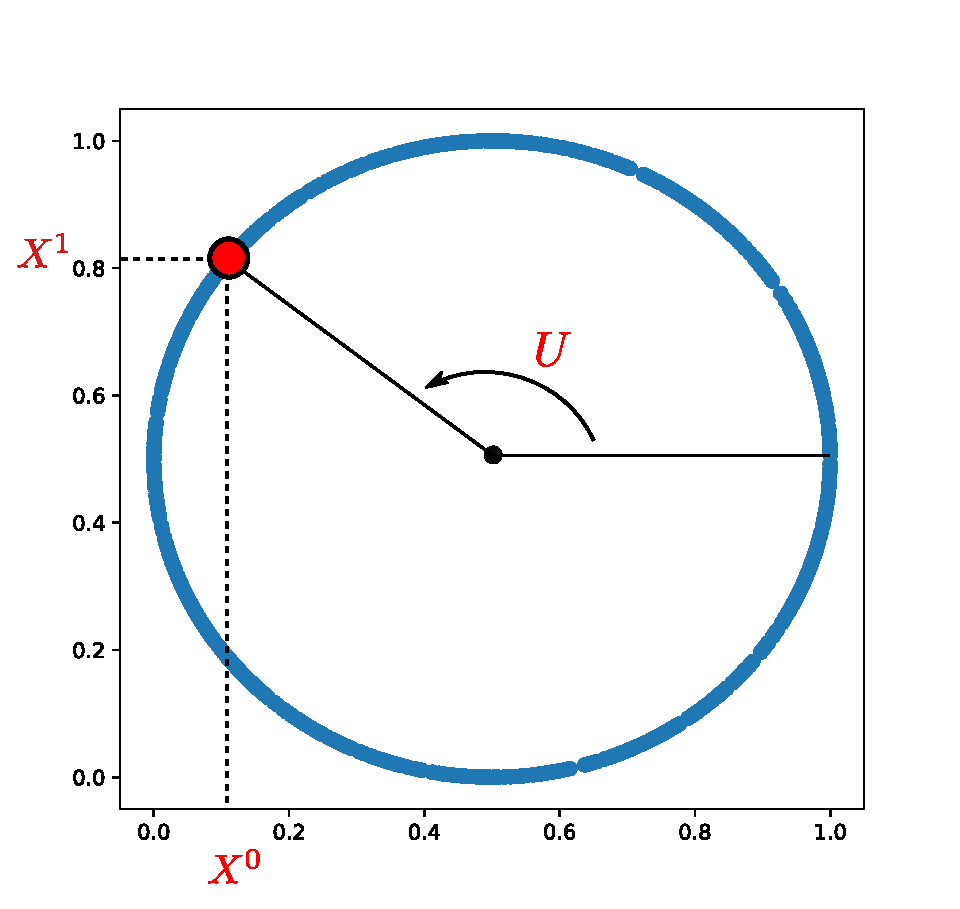
\includegraphics[width=0.6\textwidth]{cercle.pdf}
\end{minipage}
\begin{minipage}{0.5\textwidth}
\centering
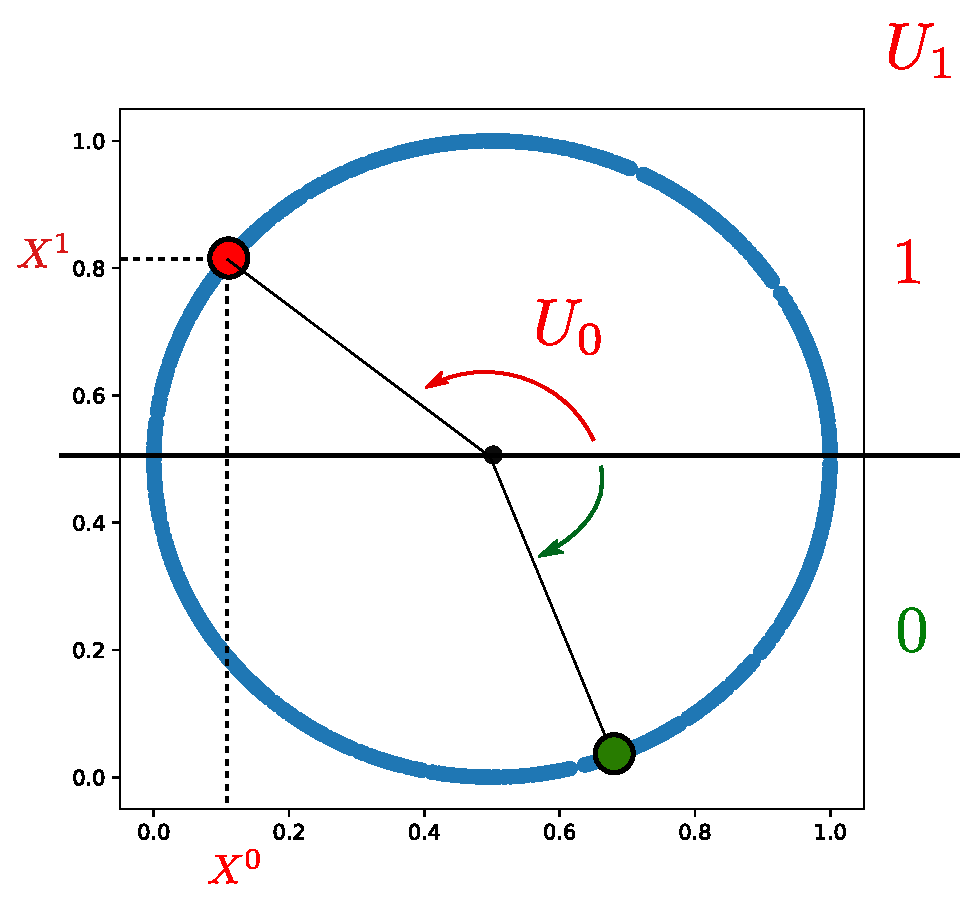
\includegraphics[width=0.6\textwidth]{cercle_2.pdf}
\end{minipage}
\caption{Exemples de paramétrisations du cercle. La paramétrisation qui traduit le plus facilement le modèle est naturellement celle dans laquelle $U$ est à valeurs réelles. Le modèle auxquelles appartiennent les modalités $X^0$ et $X^1$ est donc représenté par la variable cachée $U$.}
\end{figure}

\subsection{Représentation des éléments des cartes}



\section{Représentations graphiques}

\section{Indicateurs}


